\documentclass[a4paper]{article}
\usepackage[utf8]{inputenc}
\usepackage{titling}
\usepackage{minted}
\usepackage{fancyvrb}
\usepackage{graphicx}
\usepackage{listings}
\usepackage{float}
\usepackage[binary-units=true]{siunitx}
\IfFileExists{bookmark.sty}{\usepackage{bookmark}}{\usepackage{hyperref}}

\lstset{
	basicstyle=\ttfamily,
	columns=fullflexible,
	breaklines=true
}

\graphicspath{ {./images/} }

\newcommand{\subtitle}[1]{
  \posttitle{
    \par\end{center}
    \begin{center}\large#1\end{center}
    \vskip0.5em}
}
 
\title{MapReduce}
\subtitle{A very primitive (and flawed) implementation of MapReduce}
\author{Alexander Lampalzer}
\date{\today}

\begin{document}

\begin{titlepage}
\maketitle
\end{titlepage}

\tableofcontents
\thispagestyle{empty}
\newpage

\hypertarget{License}{%
\section{License}\label{License}}
\begin{lstlisting}
Boost Software License - Version 1.0 - August 17th, 2003

Permission is hereby granted, free of charge, to any person or organization obtaining a copy of the software and accompanying documentation covered by this license (the "Software") to use, reproduce, display, distribute, execute, and transmit the Software, and to prepare derivative works of the Software, and to permit third-parties to whom the Software is furnished to do so, all subject to the following:


The copyright notices in the Software and this entire statement, including the above license grant, this restriction and the following disclaimer, must be included in all copies of the Software, in whole or in part, and all derivative works of the Software, unless such copies or derivative works are solely in the form of machine-executable object code generated by a source language processor.

THE SOFTWARE IS PROVIDED "AS IS", WITHOUT WARRANTY OF ANY KIND, EXPRESS OR IMPLIED, INCLUDING BUT NOT LIMITED TO THE WARRANTIES OF MERCHANTABILITY,
FITNESS FOR A PARTICULAR PURPOSE, TITLE AND NON-INFRINGEMENT. IN NO EVENT SHALL THE COPYRIGHT HOLDERS OR ANYONE DISTRIBUTING THE SOFTWARE BE LIABLE
FOR ANY DAMAGES OR OTHER LIABILITY, WHETHER IN CONTRACT, TORT OR OTHERWISE 
ARISING FROM, OUT OF OR IN CONNECTION WITH THE SOFTWARE OR THE USE OR OTHER DEALINGS IN THE SOFTWARE.
\end{lstlisting}

\newpage

\hypertarget{Introduction}{%
\section{Introduction}\label{Introduction}}

The goal of this project is to create fully implement the MapReduce algorithm in cpp. It is not meant for any sort of production environment, but rather to educate the author in writing c++.

\hypertarget{technologies}{%
\subsection{Technologies}\label{technologies}}

\begin{table}[h]
	\centering
	\begin{tabular}{l|l}
		Purpose                       & Technology \\ \hline
		Build Tool				 	  & Meson	   \\
		Command line interface	      & CLI11      \\
		Configuration files           & json       \\
		Data serialization            & Protobuf   \\
		Logging                       & spdlog     \\
		Network Communication         & asio       \\
		Network Communication         & gRPC       \\
		Programming Languages		  & C++ 14, Python \\
		String Manipulation			  & fmt		   
	\end{tabular}
	\caption{This table lists all the technologies used for this project.}
\end{table}

\hypertarget{Map-Reduce-Algorithm}{%
\section{Map Reduce Algorithm}\label{Map Reduce Algorithm}}

MapReduce is an algorithm for distributed, parallel processing of data. It accomplishes this, by dividing up the input data into chunks and processing these chunks in several stages. The following graphic depicts these stages and shows what input and output are needed / provieded ny each stage.

\begin{figure}
\centering
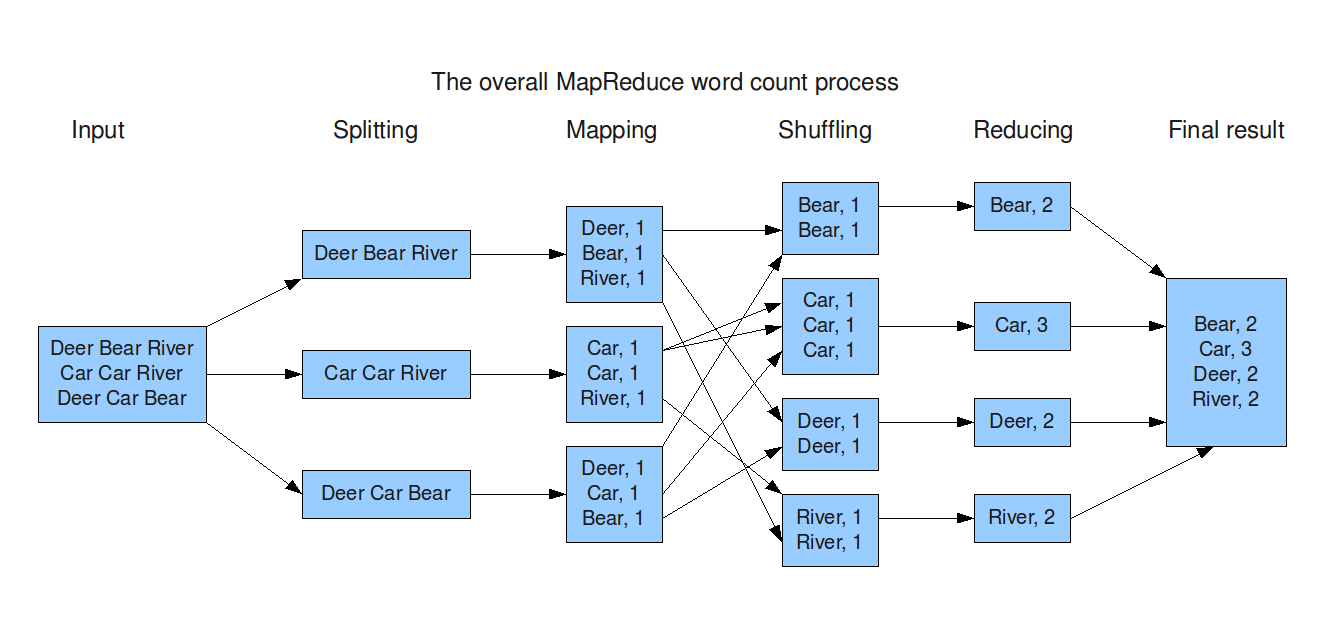
\includegraphics[width=\linewidth]{images/Phases.png}
\caption{This diagram shows the different phases of the MapReduce
algorith, as explained in the following section.}
\end{figure}

\hypertarget{stage-1-splitting}{%
\subsection{Stage 1: Splitting}\label{stage-1-splitting}}

The main goal of this stage, is to split up the input data into chunks, hence the name "Splitting". This can be accomplished in several ways. A common approach (and the approach used in this project) is to split at the end of each line. This is rather simple, however results in an increased amount of chunks, that have to be processed. Another apprach, which is used by the popular big data processing software "Hadoop" is to split the data into block of 64MB.

In this implementation, the splitting phase is realised on the client's computer, or to be more precise, in the command line interface (CLI). Data is first ingested by this cli, then splitted and finally uploaded in chunks to the master. This is primarily due to simplicity reasons.

\hypertarget{stage-2-mapping}{%
\subsection{Stage 2: Mapping}\label{stage-2-mapping}}

In it's core, this phase is quite simple: It takes input data, processes it using whatever algorithm the user intends to use and returns a list of key-value pairs - for example [(Foo, 2), (Bar, 1)].

This implementation realises the map phase, by distributing so called "jobs" to each node. A job contains a python script and the data, that needs processing. Each node writes the code to this and executes it using python3. Obviousely, this is a security risk, because running unveried code on some random machine in some data center is inherently flawed, however for reasons of simplicity in the implementation this approach was choosen.

\hypertarget{stage-3-shuffling}{%
\subsection{Stage 3: Shuffling}\label{stage-3-shuffling}}

The purpose of this stage is to organise the key-value pairs generated by mapping stage and grouping them by key. Each group is then independently sent to a node. In reality this stage is very complicated, because the cost of transferring data is high and in an optimal case, this should be minimized.

\hypertarget{stage-4-reduce}{%
\subsection{Stage 4: Reduce}\label{stage-4-reduce}}

This phase ingests the groups of data generated and applies some form of user-specified algorithm to it - in the end, the result is exactly one key-value pair for each group. These pairs are then accumalated and stored on the disk, for the user to retrieve and utilize.

\hypertarget{software-architecture}{%
\section{Software Architecture}\label{software-architecture}}

\hypertarget{communication-lifecycle}{%
\subsection{Communication / Lifecycle}\label{communication-lifecycle}}

\begin{figure}
\centering
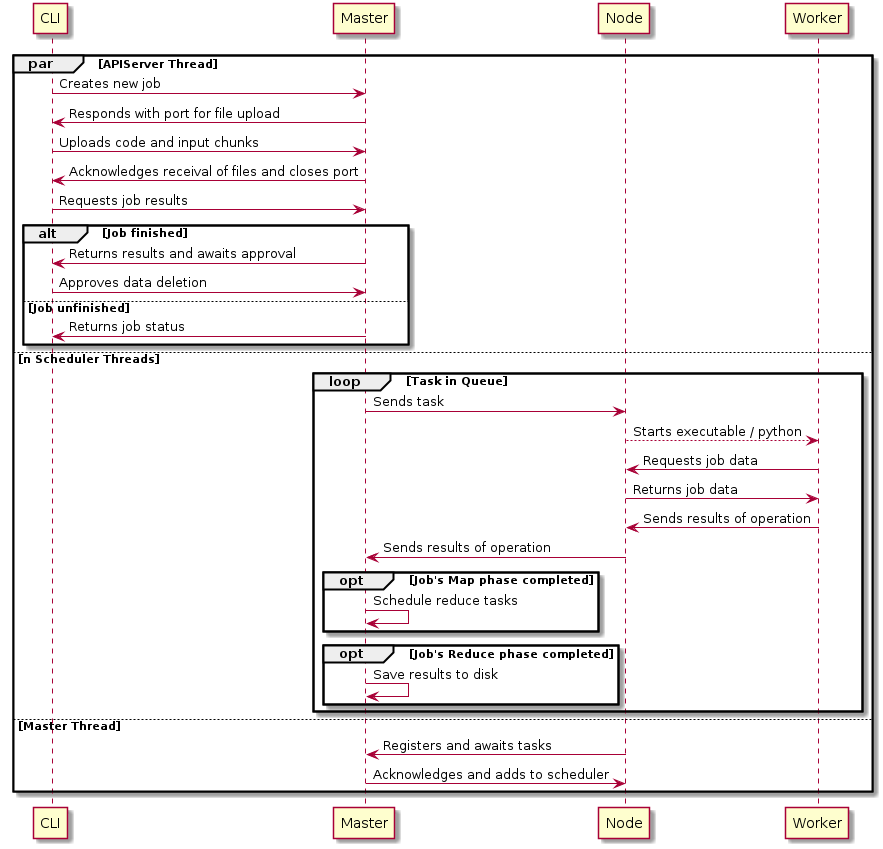
\includegraphics[width=\linewidth]{images/sequence_diagram}
\caption{This diagram depicts the messages sent between the different components of this implementation. Furthermore, it is seperated into threads, which are running simultaniousely on the Master.}
\end{figure}

This section will explain the cummunication diagram chronologically, starting at the first user input to the cli.

The first step for a user is to create a new job. This is achived, by writing a "job.json" file, as described in Section 3.1 and provide the input and this configuration file to the CLI. The CLI then goes ahead and communicates to the master, that it wishes to upload data. For the sake of minimizing impact on other user, the approach has been chosen to then open a new, sperate port on the master to receive data on. After data upload has finished, this data is ingested by the master and eventually scheduled for mapping on a Node.

Once a new node is created on the network, it registeres with the master and thus is ready to be included in task scheduling.

Each time a new task is sent to the node, the code of that particular task is written to a temporary space on the disk and executed, a new Worker has been created. This worker then goes ahead and retrives the job and it's associated data from the node, processes it and sends it back to the master, via the node.

Eventually all map task are completed, at this point the master shuffles, sorts and groups the data, to then schedule new reduce tasks. The results of this phase are stored to the disk, to be later retrieved by the user.

\hypertarget{components}{%
\subsection{Components}\label{components}}

\hypertarget{node}{%
\subsubsection{Node}\label{node}}

In comparison to the master, a node is relatively simple. A node is only able to process exactly one task at a time, however that can be multiple nodes for each computer. Optimally, the number of nodes is equal to the number of CPU cores. 

\begin{figure}
\centering
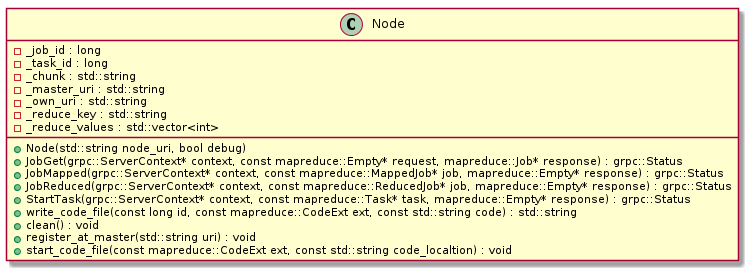
\includegraphics[width=\linewidth]{images/class_diagram_node}
\caption{This class diagram shows the relationships, methods and variables of each class of a MapReducen node}
\end{figure}

\hypertarget{master}{%
\subsubsection{Master}\label{master}}

In the diagram, the master is the central component. The APIServer is responsible of ingesting data from the CLIs, processing it and then sending it off to the master. The FIFOScheduler takes care of scheduling map and reduce jobs on all nodes - in this case FIFO stands for "First in first out", which means that in essence the tasks are put into a queue.

\begin{figure}
\centering
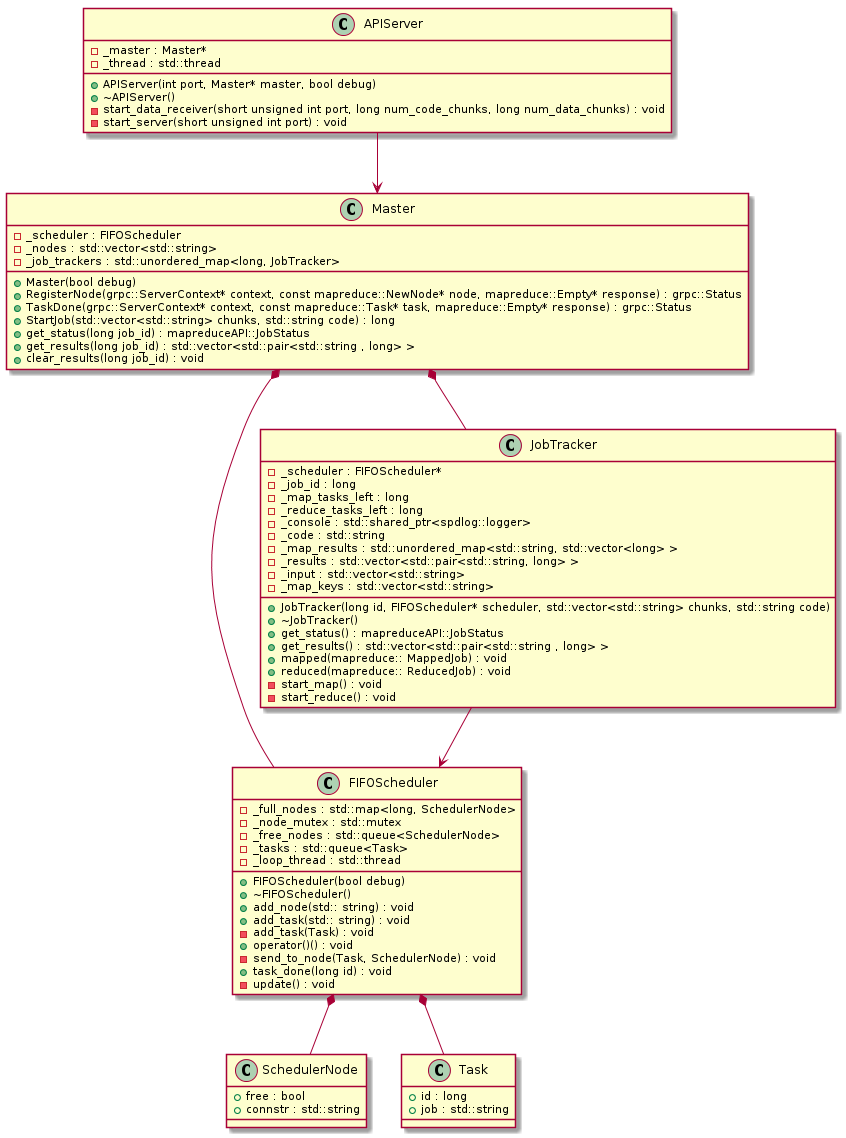
\includegraphics[width=\linewidth]{images/class_diagram_master}
\caption{This class diagram shows the relationships, methods and variables of each class of the MapReduce Master}
\end{figure}

\hypertarget{cli}{%
\subsubsection{CLI}\label{cli}}

Because of size and complexity, the CLI has not been structured in an object-oriented manner. It is relatively straight-forward with nearly no logic involved.

\hypertarget{usage-guide}{%
\section{Usage guide}\label{usage-guide}}

\hypertarget{for-end-users}{%
\subsection{For End-users}\label{for-end-users}}

\hypertarget{python-api}{%
\subsubsection{Python API}\label{python-api}}

The python API for writing MapReduce algorithms should be mostly self-explainatory, however here is one example to count word occurances.

\begin{minted}[linenos, breaklines, frame=single]{python}
from MapReduce import Worker

def map_func(chunk):
	results = []
	for word in str(chunk).split(' '):
		results.append([word, 1])

	return results

def reduce_func(key, values):
	return sum(values)

Worker(map_func, reduce_func)

\end{minted}

\hypertarget{cli-1}{%
\subsubsection{CLI}\label{cli-1}}

For interacting with the MapReduce system, a clean and easby command line interface is provided. To start a job, first of all, a job configuration file aka. job.json has to be created. It has to follow the following schema:

\begin{minted}[linenos, breaklines, frame=single]{json}
{
	"input": "shakespeare.txt",
	"split": "line",
	"code": "impl.py",
	"ip": "127.0.0.1",
	"port": "3000"
}
\end{minted}

Next, the cli needs to do it's magic. Just use \mintinline{shell}{./cli start --config job.json} to start a new job. Wait a little while, get a coffe and call  \mintinline{shell}{./cli status --id <job_id>} to retrieve either the results, or the current status of the job. That's it!

\hypertarget{for-system-administrators}{%
\subsection{For System Administrators}\label{for-system-administrators}}

Start one master by using  \mintinline{shell}{./master}- there are command line parameters provided to change the Master and API ports.
Start nodes by using  \mintinline{shell}{./node}, master IP and Port can be specified on the command line.

\end{document}

\end{document}